\documentclass[a4paper,12pt,twoside]{memoir}

% Castellano
\usepackage[spanish,es-tabla]{babel}
\selectlanguage{spanish}
\usepackage[utf8]{inputenc}
\usepackage[T1]{fontenc}
\usepackage{lmodern} % scalable font
\usepackage{microtype}
\usepackage{placeins}

\RequirePackage{booktabs}
\RequirePackage[table]{xcolor}
\RequirePackage{xtab}
\RequirePackage{multirow}

% Links
\usepackage[colorlinks]{hyperref}
\hypersetup{
	allcolors = {red}
}

% Ecuaciones
\usepackage{amsmath}

% Rutas de fichero / paquete
\newcommand{\ruta}[1]{{\sffamily #1}}

% Párrafos
\nonzeroparskip


% Imagenes
\usepackage{graphicx}
\newcommand{\imagen}[2]{
	\begin{figure}[!h]
		\centering
		\includegraphics[width=0.9\textwidth]{#1}
		\caption{#2}\label{fig:#1}
	\end{figure}
	\FloatBarrier
}

\newcommand{\imagenflotante}[2]{
	\begin{figure}%[!h]
		\centering
		\includegraphics[width=0.9\textwidth]{#1}
		\caption{#2}\label{fig:#1}
	\end{figure}
}



% El comando \figura nos permite insertar figuras comodamente, y utilizando
% siempre el mismo formato. Los parametros son:
% 1 -> Porcentaje del ancho de página que ocupará la figura (de 0 a 1)
% 2 --> Fichero de la imagen
% 3 --> Texto a pie de imagen
% 4 --> Etiqueta (label) para referencias
% 5 --> Opciones que queramos pasarle al \includegraphics
% 6 --> Opciones de posicionamiento a pasarle a \begin{figure}
\newcommand{\figuraConPosicion}[6]{%
  \setlength{\anchoFloat}{#1\textwidth}%
  \addtolength{\anchoFloat}{-4\fboxsep}%
  \setlength{\anchoFigura}{\anchoFloat}%
  \begin{figure}[#6]
    \begin{center}%
      \Ovalbox{%
        \begin{minipage}{\anchoFloat}%
          \begin{center}%
            \includegraphics[width=\anchoFigura,#5]{#2}%
            \caption{#3}%
            \label{#4}%
          \end{center}%
        \end{minipage}
      }%
    \end{center}%
  \end{figure}%
}

%
% Comando para incluir imágenes en formato apaisado (sin marco).
\newcommand{\figuraApaisadaSinMarco}[5]{%
  \begin{figure}%
    \begin{center}%
    \includegraphics[angle=90,height=#1\textheight,#5]{#2}%
    \caption{#3}%
    \label{#4}%
    \end{center}%
  \end{figure}%
}
% Para las tablas
\newcommand{\otoprule}{\midrule [\heavyrulewidth]}
%
% Nuevo comando para tablas pequeñas (menos de una página).
\newcommand{\tablaSmall}[5]{%
 \begin{table}
  \begin{center}
   \rowcolors {2}{gray!35}{}
   \begin{tabular}{#2}
    \toprule
    #4
    \otoprule
    #5
    \bottomrule
   \end{tabular}
   \caption{#1}
   \label{tabla:#3}
  \end{center}
 \end{table}
}

%
%Para el float H de tablaSmallSinColores
\usepackage{float}

%
% Nuevo comando para tablas pequeñas (menos de una página).
\newcommand{\tablaSmallSinColores}[5]{%
 \begin{table}[H]
  \begin{center}
   \begin{tabular}{#2}
    \toprule
    #4
    \otoprule
    #5
    \bottomrule
   \end{tabular}
   \caption{#1}
   \label{tabla:#3}
  \end{center}
 \end{table}
}

\newcommand{\tablaApaisadaSmall}[5]{%
\begin{landscape}
  \begin{table}
   \begin{center}
    \rowcolors {2}{gray!35}{}
    \begin{tabular}{#2}
     \toprule
     #4
     \otoprule
     #5
     \bottomrule
    \end{tabular}
    \caption{#1}
    \label{tabla:#3}
   \end{center}
  \end{table}
\end{landscape}
}

%
% Nuevo comando para tablas grandes con cabecera y filas alternas coloreadas en gris.
\newcommand{\tabla}[6]{%
  \begin{center}
    \tablefirsthead{
      \toprule
      #5
      \otoprule
    }
    \tablehead{
      \multicolumn{#3}{l}{\small\sl continúa desde la página anterior}\\
      \toprule
      #5
      \otoprule
    }
    \tabletail{
      \hline
      \multicolumn{#3}{r}{\small\sl continúa en la página siguiente}\\
    }
    \tablelasttail{
      \hline
    }
    \bottomcaption{#1}
    \rowcolors {2}{gray!35}{}
    \begin{xtabular}{#2}
      #6
      \bottomrule
    \end{xtabular}
    \label{tabla:#4}
  \end{center}
}

%
% Nuevo comando para tablas grandes con cabecera.
\newcommand{\tablaSinColores}[6]{%
  \begin{center}
    \tablefirsthead{
      \toprule
      #5
      \otoprule
    }
    \tablehead{
      \multicolumn{#3}{l}{\small\sl continúa desde la página anterior}\\
      \toprule
      #5
      \otoprule
    }
    \tabletail{
      \hline
      \multicolumn{#3}{r}{\small\sl continúa en la página siguiente}\\
    }
    \tablelasttail{
      \hline
    }
    \bottomcaption{#1}
    \begin{xtabular}{#2}
      #6
      \bottomrule
    \end{xtabular}
    \label{tabla:#4}
  \end{center}
}

%
% Nuevo comando para tablas grandes sin cabecera.
\newcommand{\tablaSinCabecera}[5]{%
  \begin{center}
    \tablefirsthead{
      \toprule
    }
    \tablehead{
      \multicolumn{#3}{l}{\small\sl continúa desde la página anterior}\\
      \hline
    }
    \tabletail{
      \hline
      \multicolumn{#3}{r}{\small\sl continúa en la página siguiente}\\
    }
    \tablelasttail{
      \hline
    }
    \bottomcaption{#1}
  \begin{xtabular}{#2}
    #5
   \bottomrule
  \end{xtabular}
  \label{tabla:#4}
  \end{center}
}



\definecolor{cgoLight}{HTML}{EEEEEE}
\definecolor{cgoExtralight}{HTML}{FFFFFF}

%
% Nuevo comando para tablas grandes sin cabecera.
\newcommand{\tablaSinCabeceraConBandas}[5]{%
  \begin{center}
    \tablefirsthead{
      \toprule
    }
    \tablehead{
      \multicolumn{#3}{l}{\small\sl continúa desde la página anterior}\\
      \hline
    }
    \tabletail{
      \hline
      \multicolumn{#3}{r}{\small\sl continúa en la página siguiente}\\
    }
    \tablelasttail{
      \hline
    }
    \bottomcaption{#1}
    \rowcolors[]{1}{cgoExtralight}{cgoLight}

  \begin{xtabular}{#2}
    #5
   \bottomrule
  \end{xtabular}
  \label{tabla:#4}
  \end{center}
}




\graphicspath{ {./img/} }

% Capítulos
\chapterstyle{bianchi}
\newcommand{\capitulo}[2]{
	\setcounter{chapter}{#1}
	\setcounter{section}{0}
	\chapter*{#2}
	\addcontentsline{toc}{chapter}{#2}
	\markboth{#2}{#2}
}

% Apéndices
\renewcommand{\appendixname}{Apéndice}
\renewcommand*\cftappendixname{\appendixname}

\newcommand{\apendice}[1]{
	%\renewcommand{\thechapter}{A}
	\chapter{#1}
}

\renewcommand*\cftappendixname{\appendixname\ }

% Formato de portada
\makeatletter
\usepackage{xcolor}
\newcommand{\tutor}[1]{\def\@tutor{#1}}
\newcommand{\course}[1]{\def\@course{#1}}
\definecolor{cpardoBox}{HTML}{E6E6FF}
\def\maketitle{
  \null
  \thispagestyle{empty}
  % Cabecera ----------------
\noindent
\includegraphics[width=\textwidth]{cabecera}\vspace{1cm}%
  \vfill
  % Título proyecto y escudo informática ----------------
  \colorbox{cpardoBox}{%
    \begin{minipage}{.8\textwidth}
      \vspace{.5cm}\Large
      \begin{center}
      \textbf{TFG del Grado en Ingeniería Informática}\vspace{.6cm}\\
      \textbf{\LARGE\@title{}}
      \end{center}
      \vspace{.2cm}
    \end{minipage}

  }%
  \hfill\begin{minipage}{.20\textwidth}
    
\includegraphics[width=\textwidth]{escudoInfor}
  \end{minipage}
  \vfill
  % Datos de alumno, curso y tutores ------------------
  \begin{center}%
  {%
    \noindent\LARGE
    Presentado por \@author{}\\ 
    en Universidad de Burgos --- \@date{}\\
    Tutor: \@tutor{}\\
  }%
  \end{center}%
  \null
  \cleardoublepage
  }
\makeatother


% Datos de portada
\title{título del TFG \\Documentación Técnica}
\author{nombre alumno}
\tutor{nombre tutor}
\date{\today}

\begin{document}

\maketitle



\cleardoublepage



%%%%%%%%%%%%%%%%%%%%%%%%%%%%%%%%%%%%%%%%%%%%%%%%%%%%%%%%%%%%%%%%%%%%%%%%%%%%%%%%%%%%%%%%



\frontmatter


\clearpage

% Indices
\tableofcontents

\clearpage

\listoffigures

\clearpage

\listoftables

\clearpage

\mainmatter

\appendix

\apendice{Plan de Proyecto Software}\label{ch:plan}

\section{Introducción} \label{sec:plan-intro}
En el este capitulo se describe el resultado obtenido tras la planificación del
proyecto \extranjerismo{software}.

La planificación toma dos vertientes. Primero se analiza la planificación 
temporal del proyecto. En esta fase se determina de manera general la cantidad
y el tipo de tareas a realizar. Una vez descompuestas las tareas en subtareas
se puede estimar el tiempo requerido para la realización de cada subtarea.
Y a su vez, tareas y el proyecto completo.

Cabe destacar que la planificación inicial puede sufrir desvíos que impliquen
modificarla a lo largo del desarrollo. Al usar la metodología Scrum, tras
terminar cada \extranjerismo{sprint} se puede evaluar si el desarrollo se está
ciñendo a lo esperado.

Por otro parte se realiza un análisis de la viabilidad del proyecto. En todo
desarrollo se ven involucrados diferentes factores que pueden determinar la
viabilidad o no del proyecto. Los circunstancias analizadas son la viabilidad
económica y la viabilidad legal. Se busca conocer el coste económico estimado
en la realización del proyecto. Y también se quiere analizar el tipo de
licenciamiento \extranjerismo{software} que afecta al proyecto. Así como las
licencias que se van a asignar.

\section{Planificación temporal} \label{sec:plan-temporal}

Como se han empleado la metodología Scrum, la planificación se ha realizado
entorno a los \extranjerismo{sprints}. En la planificación inicial se
establecieron de forma general el número de \extranjerismo{sprints} y el
objetivo de cada uno de ellos.

La duración asignada a los \extranjerismo{sprint} se extendía de una semana a un
mes. Como se ha usado ZenHub para la gestión del proyecto, se pudo asignar una
estimación a las tareas en forma de \extranjerismo{Story points}.
La puntuación abarca desde un punto, para las tareas más simples y breves;
hasta los cuarenta puntos, de las tareas más complejas y que podían ocupar la
mayor parte del tiempo del \extranjerismo{sprint}.

La planificación inicial fue la siguiente:
\begin{itemize}
  \item \extranjerismo{Sprint} 1 Estudio e investigación
  \item \extranjerismo{Sprint} 2 Comunicarse con la placa usando TCP/IP 
  \item \extranjerismo{Sprint} 3 Implementar las funciones del 
    \extranjerismo{hardware}
  \item \extranjerismo{Sprint} 4 Desarrollar la aplicación web
  \item \extranjerismo{Sprint} 5 Finalizar la documentación de la memoria
  \item \extranjerismo{Sprint} 6 Finalizar la documentación de los apéndices
\end{itemize}

A continuación se muestra la planificación específica de cada
\extranjerismo{sprints} mostrando sus objetivos, las tareas que los componen,
la estimación de cada tarea y el resultado obtenido tras su finalización.

\clearpage

\subsection{Plan del \extranjerismo{Sprint} 1} \label{sec:plan-s1}
La estimación del \extranjerismo{sprint} se estableció en una semana de
duración. Con en este \extranjerismo{sprint} se realizaba la primera toma de
contacto con el proyecto. Las tareas a realizar giraban en torno al estudio de
la placa de desarrollo y sobre la elección del resto de herramientas, técnicas y
metodologías.

Acciones a realizar en este \extranjerismo{sprint}:
\begin{itemize}
  \item Estudio de las herramientas de trabajo.
  \item Investigación sobre la placa de desarrollo FRDM-K64F.
  \item Estudio sobre FreeRTOS y lwIP.
  \item Elección de las herramientas y \extranjerismo{software} a emplear.    
\end{itemize}

\imagen{sprint1}{Tareas planificadas para el Sprint 1}

Las tareas del \extranjerismo{sprint} se realizaron según lo previsto al plan.
El estudio sobre el IDE resulto la tarea más compleja según lo estimado al 
tener que usar la nuevas herramientas del IDE. Al terminar sin imprevistos,
se pudo planear las tareas del siguiente \extranjerismo{sprint}.

\clearpage

\subsection{Plan del \extranjerismo{Sprint} 2} \label{sec:plan-s2}
La estimación del \extranjerismo{sprint} se estableció en una semana de
duración. Conociendo las herramientas con la que trabajar en este
\extranjerismo{sprint} se pretendía comenzar el desarrollo. 

Acciones a realizar en este \extranjerismo{sprint}:
\begin{itemize}
  \item Creación del proyecto de trabajo.
  \item Realizar las primeras comunicaciones TCP/IP.  
  \item Realizar las operaciones remotas con la placa.
\end{itemize}

\imagen{sprint2}{Tareas planificadas para el Sprint 2}

El \extranjerismo{sprint} se completó de acuerdo a lo previsto. Aunque se 
estimó que la configuración del proyecto y el uso de lwIP no serían muy
complejos su ejecución resultó más compleja, sin embargo, se realizó a tiempo
para planificar y empezar el siguiente \extranjerismo{sprint}.

\clearpage

\subsection{Plan del \extranjerismo{Sprint} 3} \label{sec:plan-s3}
De nuevo, la estimación del \extranjerismo{sprint} se estableció en una semana
de duración. Como era posible enviar datos a la placa, en este
\extranjerismo{sprint} se deseaba ampliar la funcionalidad de la placa K64F
con el uso de sus periféricos.

Acciones a realizar en este \extranjerismo{sprint}:
\begin{itemize}
  \item Configurar los LED RBG y realizar la programación para su manejo remoto.
  \item Configurar el LCD y realizar la programación para su manejo remoto. 
  \item Configurar los LED PWM y realizar la programación para su manejo remoto.
\end{itemize}

\imagen{sprint3}{Tareas planificadas para el Sprint 3}

Este fue el primer \extranjerismo{sprint} en desviarse de lo previsto. 
La configuración del bus I\textsuperscript{2}C y la adaptación de la librería
del LCD requirió mucho más tiempo de lo estimado. Al aumentar la duración
de este \extranjerismo{sprint} se tuvo que retrasar el inicio del siguiente.
Tras terminarlo, se pudieron planificar las tareas siguientes.

\clearpage

\subsection{Plan del \extranjerismo{Sprint} 4} \label{sec:plan-s4}
Con el cambio al desarrollo de la aplicación web y teniendo en cuenta la
posibilidad de nuevos retrasos como en el \extranjerismo{sprint} anterior,
en este se decidió aumentar la planificación temporal a dos semanas.

Acciones a realizar en este \extranjerismo{sprint}:
\begin{itemize}
  \item Analizar el intercambio de datos necesario entre app y placa.
  \item Diseñar las interfaces de la aplicación. 
  \item Implementar las funciones de comunicación.
  \item Desarrollar la interfaz web.
\end{itemize}

\imagen{sprint4}{Tareas planificadas para el Sprint 4}

El desarrollo de la aplicación presentó varios desafíos, el aprendizaje y 
programación con CSS fueron algunos de ellos. Pese a todo la duración no 
se desvió demasiado de lo previsto.

\clearpage

\subsection{Plan del \extranjerismo{Sprint} 5} \label{sec:plan-s5}
Terminados el desarrollo del \extranjerismo{sofware} de la placa y 
el desarrollo de la aplicación web faltaba completar la documentación del 
proyecto. Inicialmente se planificó que el \extranjerismo{sprint}
tendría una duración de dos semanas.

Acciones a realizar en este \extranjerismo{sprint}:
\begin{itemize}
  \item Completar los distintos capítulos de la memoria.
\end{itemize}

\imagen{sprint5}{Tareas planificadas para el Sprint 5}

El tiempo dedicado a preparase para usar \LaTeX{} fue erróneamente subestimado.
Al tener que dedicar varios días más de lo previsto en este punto, el último
\extranjerismo{sprint} tuvo que empezar jornadas un tiempo más tarde.

\clearpage

\subsection{Plan del \extranjerismo{Sprint} 6} \label{sec:plan-s6}
Completada la memoria se completaría la información proporcionada con una
serie de anexos. La duración se estimó en una semana debido a los plazos
temporales restantes.

Acciones a realizar en este \extranjerismo{sprint}:
\begin{itemize}
  \item Completar los distintos apéndices.
\end{itemize}

\imagen{sprint6}{Tareas planificadas para el Sprint 6}

Completada la documentación se pudo proceder a la conclusión satisfactoria
del proyecto.

\clearpage

\subsection{Planificación temporal completa} \label{sec:plan-total}
En las siguientes páginas se pueden comparar la planificación inicial
y la final.

\imagen{tareas1}{Sprints planificados inicialmente}

\imagen{tareas2}{Sprints planificados finalmente}

\figuraApaisadaSinMarco{0.7}{gantt1}{Diagrama de Gantt de la planificación
inicial}{fig:gantt1}{}

\figuraApaisadaSinMarco{0.8}{gantt2}{Diagrama de Gantt de la planificación
final}{fig:gantt2}{}

\newpage

\section{Estudio de viabilidad}
\subsection{Viabilidad económica}
Para determinar la viabilidad económica del proyecto, en este apartado se
computan los gastos previstos durante el desarrollo y los posibles beneficios
si los hubiera. De haberse realizado en una empresa, los costes se calcularían
como se muestra a continuación.

\subsubsection{Coste de personal}
El desarrollo se ha realizado por una sola persona en un tiempo aproximado de
90 días, así que, todos los costes de personal son relativos a esa única
persona. El salario mensual bruto asignado ha sido de \EUR{2200}.

De manera simplificada, el salario neto se puede calcular de la siguiente forma:
\begin{equation} \label{eq:salario}
  salario\ bruto - IRFP - SS = salario\ neto
\end{equation}

Por tanto, para un mes dado el salario neto a percibir sería el siguiente:
\begin{equation} \label{eq:salario}
  2200\text{\euro} - 14\% \footnote{Usado el tramo más alto de la
  escala autonómica de Castilla y León aplicable a la base liquidable
  general del IRPF \cite{webpage:cyl}}
  - 6,35\% = 1752,30\text{\euro}
\end{equation}

\subsubsection{Costes pertenecientes a la SS}
Sobre el salarios se producen ciertas retenciones y pagos a la Seguridad Social,
algunos conceptos corren a cargo de la empresa contratante y otros
por parte del trabajador. A continuación de calculan sus importes.

Para el cálculo de la retenciones se toma como referencia la tablas de bases
de cotización ofrecida por la propia Seguridad Social \cite{webpage:ss}. En
concreto datos del primer grupo de cotización: ``Ingenieros y Licenciados. 
Personal de alta dirección no incluido en el artículo 1.3.c)
del Estatuto de los Trabajadores''. Este grupo tiene unas bases mínimas de
\EUR{1466,40}/mes. Y unas máximas de \EUR{4070,10}/mes.

\tablaSmallSinColores{Costes pertenecientes a la SS}{l l l}{costes-ss}
{\multicolumn{1}{l}{Concepto} & Empresa & Trabajador\\}
{
  Contingencias comunes & 23,60\% & 4,70\%\\
  Desempleo             &  5,50\% & 1,55\%\\
  FOGASA                &  0,20\% & 0,00\%\\
  Formación             &  0,60\% & 0,10\%\\
  \textbf{Total}        & \textbf{29,9\%} & \textbf{6,35\%}\\
}

Por consiguiente, la empresa tendría que añadir a los costes el 23,9\% del
salario del trabajador y el trabajador sufriría una retención del 6,35\%.

\subsubsection{Coste total de personal}
El coste total se calcula con la siguiente fórmula:
\begin{equation} \label{eq:salario}
  (salario\ mensual + retenciones\ ss) \times n^{o}\ meses = coste\ total
\end{equation}

De modo que el coste total se obtiene así:
\begin{equation} 
  (2200\text{\euro} + 657,8\text{\euro}) \times 3 = 8573,4\text{\euro}
\end{equation}

La tabla siguiente tabla recoge diferentes costes asociados al personal y 
su coste total.

\tablaSmallSinColores{Coste total de personal}{l l}{personal}
{\multicolumn{1}{l}{Concepto} & Coste\\}
{
  Salarios          & \EUR{2200}\\
  Seguridad Social  & \EUR{657,8}\\
  Meses             & 3 meses\\
  \textbf{Total}    & \textbf{\EUR{8573,4}}\\
}

\subsubsection{Coste del \extranjerismo{hardware}}
Para realizar el desarrollo se precisa contar son varios dispositivos. Aunque
en la Ley del Impuesto sobre Sociedades \cite{webpage:is} se permite un máximo
de 8 años para amortizar equipos para procesos de información, se considera la
que renovación de \extranjerismo{hardware} se produce en un periodo más corto de
4 años. Así pues, la amortización se calcula en función de esos 4 años.

El coste mensual de un dispositivo se calcula así:
\begin{equation} \label{eq:coste-hw}
  coste\ del\ dispositivo\ /\ periodo\ de\ amortización\ (en\ meses)
\end{equation}

Por lo tanto, el coste de un dispositivo es el siguiente:
\begin{equation} \label{eq:coste-amor-hw}
  coste\ mensual\ amortizado\ \times n^{o} meses\
\end{equation}

En el desarrollo solo se va a necesitar una estación de trabajo, así pues, el
coste total del \extranjerismo{hardware} es el mostrado en la tabla a
continuación.

\tablaSmallSinColores{Coste del \extranjerismo{hardware}}{l l l}{coste-hw}
{\multicolumn{1}{l}{\extranjerismo{Hardware}} & Coste & Coste amortizado\\}
{
  Estación de trabajo & \EUR{1250} & \EUR{104,16}\\
  \textbf{Total}      & \EUR{1250} & \textbf{\EUR{104,16}}\\
}

\subsubsection{Coste del \extranjerismo{software}}
El desarrollo necesita de varios programas y aplicaciones. De igual manera que
el \extranjerismo{hardware}, la Ley del Impuesto sobre Sociedades
\cite{webpage:is} indica el máximo de años para realizar la amortización.
En sistemas y programas informáticos es de 6 años. Pero coincidiendo con el
periodo de renovación del \extranjerismo{hardware}, la amortización se calcula
en un periodo menor de 4 años.

Las fórmulas para calcular las amortizaciones son equivalentes a las usadas
en el \extranjerismo{harware} \ref{eq:coste-hw} y \ref{eq:coste-amor-hw}.

Otra parte de \extranjerismo{software} se emplea bajo suscripción, en los
cálculos solo se computa el coste de los meses que se usó dicha suscripción.

Hay que tener en cuenta, que gran parte del \extranjerismo{software} utilizado
se publica bajo licencias que permiten su uso sin coste y que gracias a esto se
reducen significativamente los costes del \extranjerismo{software}.
En consecuencia solo se calculan los costes del \extranjerismo{software} que no
es gratuito.

\tablaSmallSinColores{Coste del \extranjerismo{software}}{l l l}{coste-sw}
{\multicolumn{1}{l}
{\extranjerismo{Software}}              & Coste        & Coste amortizado\\}
{
  Windows 10 Pro\cite{webpage:win10pro} & \EUR{259}    & \EUR{21,58}\\
  Office 365\cite{webpage:office365}    & \EUR{126}    & \EUR{31,5}\\
  Adobe CC\cite{webpage:adobecc}        & \EUR{359,88} & \EUR{89,97}\\
  \textbf{Total}                        & \EUR{744,88} & \textbf{\EUR{143,05}}\\
}

\subsubsection{Coste del sistema empotrado}
El sistema empotrado se ha realizado con la ayuda de diversos componentes que
también tienen unos costes de adquisición asociados.

\tablaSmallSinColores{Coste del SE}{l l}{coste-se}
{\multicolumn{1}{l}
{Componente}                                     & Coste        \\}
{ 
  Placa FRDM-K64F\cite{webpage:k64f}             & \EUR{32,52} \\
  Placa Arduino Basic I/O\cite{webpage:basic-io} & \EUR{19,00} \\
  Pantalla LCD\cite{webpage:lcd}                 & \EUR{8,91}  \\
  Placas de pruebas\cite{webpage:placas}         & \EUR{12,24} \\
  Cables puente\cite{webpage:cables}             & \EUR{4,98}  \\
  Cable de par trenzado\cite{webpage:rj45}       & \EUR{4,88}  \\
  \textbf{Total}                                 & \textbf{\EUR{82,53}} \\
}

\subsubsection{Coste total del proyecto}
Sumando todos los costes anteriores se puede calcular el coste total de todo
el proyecto.

\tablaSmallSinColores{Coste total del proyecto}{l l}{coste-total}
{\multicolumn{1}{l}
{Tipo de coste}            & Coste        \\}
{ 
  Personal                 & \EUR{8573,4} \\
  \extranjerismo{Hardware} & \EUR{104,16} \\
  \extranjerismo{Software} & \EUR{143,05} \\
  Componentes del SE       & \EUR{82,53}  \\
  \textbf{Total}           & \textbf{\EUR{8903,14}} \\
}

\subsubsection{Beneficios del proyecto}
El código fuente del sistema empotrado (SE)y de la aplicación web se encuentran
disponibles abiertamente. Además, el SE tampoco tiene definida una función
claramente comercial. Por ello, no se considera que el proyecto
pueda tener un beneficio económico directo.

Esto tampoco quiere decir que los gastos se hagan a fondo perdido. Más bien,
se pueden considerar los gastos como una inversión en investigación y formación.
Competencias que permitirán en el futuro crear nuevos SE que rentabilicen todos
los costes.

\subsection{Viabilidad legal}
Al desarrollar un \extranjerismo{software} hay que tener en consideración
las implicaciones legales que se presental al usar \extranjerismo{software}
de terceros.

Las licencias sirven como instrumento para establecer los términos y condiciones
en los que se pueden utilizar el \extranjerismo{software} licenciado. Para
poder definir que licencias usar en el proyecto es necesario conocer las
licencias utilizadas y la restricciones que pueden imponer.

\subsubsection{Licencias utilizadas en el desarrollo del SE}
Para desarrollar el \extranjerismo{software} de la placa se ha utilizado
de código fuente de terceros que se describe a continuación.
\begin{itemize}
  \item El código generado por MCUXpresso se proporciona bajo la licencia
  ``The 3-Clause BSD License'' (BSD-3), también conococida como la
  ``New BSD License''o ``Modified BSD License''.
  \item Otra parte del código generado por MCUXpress se licencia con 
  ``The Clear BSD License''. La licencia es similar a BSD-3, pero indica
  expresamente que no se conceden derechos sobre patentes.
  \item El código perteneciente a FreeRTOS es propiedad de Amazon.com, Inc.
  Se permite el uso, copia, modificación, publicación, distribución, volver a
  licenciar y comercializar, manteniendo siempre el aviso de derechos de autor.
  \item El código de lwIP se entrega con la licencia BSD-3.
  \item Parte del código relacionado con el procesador de la placa pertenece a
  ARM Limited. El código se proporciona con la licencia Apache 2.0.
\end{itemize}

Así pues, se encuentran licencias que permiten el uso, copia, modificación y 
redistribución del código. Como BSD-3 o Apache 2.0

\subsubsection{Licencia para el SE}
Teniendo en cuanta que el código fuente del \extranjerismo{software} del SE
se pretende que sea abierto, se va a utilizar una licencia en línea con las
mostradas anteriormente.

En concreto se va a emplear la licencia Apache 2.0. Sus características 
principales se pueden ver resumidas en la siguiente tabla.

\tablaSmallSinColores{Licencia Apache 2.0}{l l l l}{apache}
{\multicolumn{1}{l}
{Permisos}        & Condiciones                & Limitaciones    \\}
{ 
  Uso comercial   & Aviso de licencia          & Responsabilidad           \\
  Distribución    & y derechos de autor        & Uso de marcas registradas \\
  Modificación    & Declaración de los cambios & Garantía                  \\ 
  Uso de patentes \\
  Uso privado     \\
}

\subsubsection{Licencia para la aplicación web}
En el caso de la aplicación web no se ha requerido de bibliotecas o librerías
de terceros como en el caso del SE. De igual forma que el SE, la aplicación web
se licencia con Apache 2.0

\subsubsection{Aviso de Apache}
Para aplicar la licencia Apache \cite{webpage:apache2-apply} es necesario
adjuntar un archivo de texto con la licencia con el nombre ``LICENSE''
en el directorio raíz del proyecto. El archivo de texto se puede copiar
desde su propia web \cite{webpage:apache2-license}.

En caso de ser necesario, se incluirá un fichero llamado ``NOTICE'' en el mismo 
directorio que la licencia que contenga información adicional.

Por último, el texto a continuación será incluido en todos los ficheros 
fuente. Se tiene que añadir como comentario en el comienzo del fichero,
sustituyendo el texto entre corchetes por el nombre del autor y por la fecha
que correspondan.

\begin{quotation}
  Copyright [yyyy] [name of copyright owner] \bigskip

  Licensed under the Apache License, Version 2.0 (the "License");
  you may not use this file except in compliance with the License.
  You may obtain a copy of the License at \bigskip
  
  \quad http://www.apache.org/licenses/LICENSE-2.0 \bigskip

  Unless required by applicable law or agreed to in writing, software
  distributed under the License is distributed on an ``AS IS'' BASIS,
  WITHOUT WARRANTIES OR CONDITIONS OF ANY KIND, either express or implied.
  See the License for the specific language governing permissions and
  limitations under the License.
\end{quotation}


\subsubsection{Licencia para la documentación}
Para el licenciamiento de la documentación se opta por otro tipo de licencia
más adecuada al tipo de obra. La licencia escogida es
Creative Commons Atribución 4.0 Internacional (CC BY 4.0) \cite{webpage:cc}.

Esta licencia permite que la obra sea compartida libremente. Puede ser copiada
y redistribuida en cualquier medio o formato. También se puede reeditar,
transformar y crear obras derivadas a partir de la obra original, incluso
comercialmente. Solo se requiere la atribución de la autoría original.

\tablaSmallSinColores{Licencia CC BY 4.0}{l l l l}{ccby4}
{\multicolumn{1}{l}
{Permisos}      & Condiciones                & Limitaciones    \\}
{ 
  Distribución  & Crédito al autor           & Responsabilidad           \\  
  Modificación  & Aviso de licencia          & Uso de patentes           \\
  Uso privado   & y derechos de autor        & Uso de marcas registradas \\
  Uso comercial & Declaración de los cambios & Garantía                  \\ 
}

El uso de la licencia se indica con la siguiente imagen y texto:

\begin{figure}[H]
  \centering
  
\includegraphics[width=0.2\textwidth]{ccby}
  \label{fig:ccby}
\end{figure}
\begin{center}
  Este obra está bajo una
\href{https://creativecommons.org/licenses/by/4.0/}
{licencia de Creative Commons Reconocimiento 4.0 Internacional}.
\end{center}

\apendice{Especificación de Requisitos}

\section{Introducción}

\section{Objetivos generales}

\section{Catalogo de requisitos}

\section{Especificación de requisitos}



\apendice{Especificación de diseño} \label{ch:design}

\section{Introducción} \label{sec:design-intro}
Tras recoger las especificaciones de los requisitos del \sw{} se 
puede comenzar con la especificación del diseño. Este apéndice detalla
las soluciones tomadas respecto al diseño del \sw{}.

Con el diseño del \sw{} se trata de dar respuesta a cuestiones relativas a los
datos, y su representación; las división lógica en módulos, y su funcionamiento
interno; y como estructurar el \sw{} arquitectónicamente.

\subsection{Ámbito del \sw{}} \label{sec:design-ambito}
El \sw{} a desarrollar debe permitir a un usuario operar con un
sistema empotrado de forma remota a través de una aplicación web. Al ser
entidades tan diferenciadas, tanto el sistema empotrado como la aplicación web
tienen que contar con \sw{} propio y específico a cada plataforma.

El \sw{} del sistema empotrado tiene que residir en el propio sistema. Con su
ejecución se pretende actuar sobre el \hw{} habilitado a tal fin.

En cuanto al \sw{} de la aplicación web, ejecutado en un servidor de aplicaciones, va a
servir como interfaz de usuario frente al sistema empotrado que le va a permitir
ordenar la ejecución de las funciones del sistema empotrado.



\section{Diseño de datos} \label{sec:design-datos}
Para que la aplicación web pueda ordenar al sistema empotrado actuar de una
determinada manera se precisa de la transmisión de unos comandos concretos. En
consecuencia, se tiene que definir la estructura de los comandos para que ambos
\extranjerismo{softwares} sean capaces de entenderse.


\subsection{Transferencia de los comandos} \label{sec:design-transferencia}
Los comandos van a ser transferidos usando el protocolo Transmission Control
Protocol (TCP). El protocolo está orientado a la conexión y se encarga de
establecerla la comunicación mediante unos mensajes de sincronización (SYN) y
reconocimiento (ACK), como se puede ver en \ref{fig:tcp}.

\begin{figure}[!h]
  \centering
  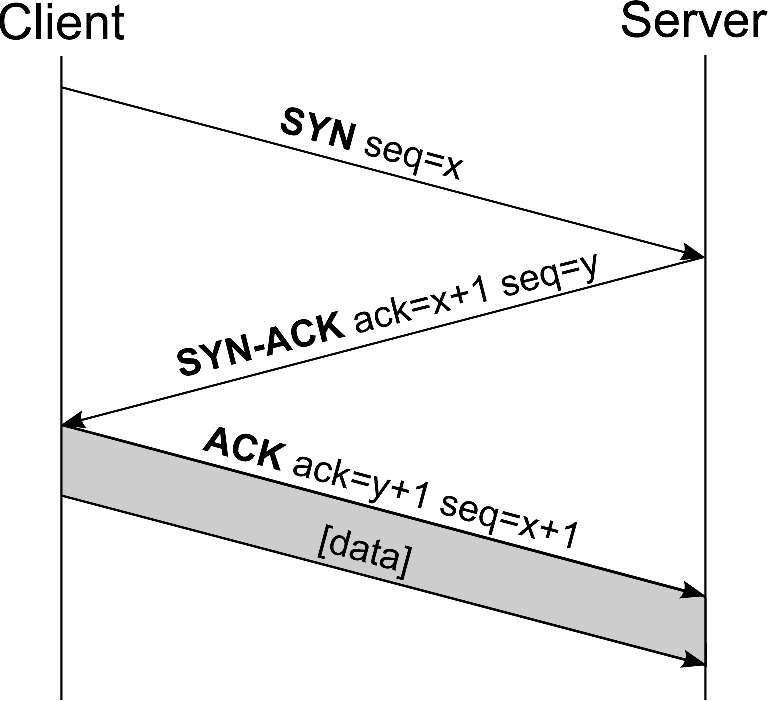
\includegraphics[width=0.6\textwidth]{tcp}
  \caption{Conexión TCP \cite{webpage:tcp-handshake}} \label{fig:tcp}
\end{figure}

Aprovechando que el protocolo TCP se encarga establecer una conexión fiable,
se delega en él el establecimiento de la conexión y los comandos serán enviados
después encapsulados dentro de segmentos TCP.


\subsection{Comando LED} \label{sec:design-datos-led}
Con este comando se indica al sistema empotrado que muestre una luz con el color
indicado. Hay un LED para cada uno de los tres colores primarios: rojo, verde y
azul. Aunque los LED pueden encenderse individualmente, encendiéndolos
simultáneamente se pueden combinar los colores primarios y generar otros
nuevos. Los colores obtenidos por adición son el cian, magenta, amarillo y
blanco. Además, debe ser posible que los LED se apaguen y dejen de iluminar.

Para conseguir lo anterior, el nombre del comando refleja la alusión a los LED
RGB. El comando se acompaña de un argumento que especifica el color concreto a
iluminar. Para ayudar a diferenciar el comando del argumento se ubica un carácter
separador.

\tablaSmallSinColores{Comando LED}{l c c c c}{comando-led}
{\multicolumn{1}{l}{Color} & Comando & Separador & Argumento & Comando resultante\\}
{
  Rojo     & led & : & r & led:r \\
  Verde    & led & : & g & led:g \\
  Azul     & led & : & b & led:b \\
  Cian     & led & : & c & led:c \\
  Magenta  & led & : & m & led:m \\
  Amarillo & led & : & y & led:y \\
  Blanco   & led & : & w & led:w \\
  No color & led & : & o & led:o \\
}


\subsection{Comando MSG} \label{sec:design-datos-msg}
Este comando indica al sistema empotrado que muestre una cadena de caracteres
en la pantalla LCD. Como la pantalla tiene dos líneas, se necesita indicar
la línea donde mostrar el texto.

El nombre del comando refleja que trata con los mensajes de texto. El comando
se acompaña de un argumento que especifica la línea donde escribir la cadena de
caracteres. Después se añade otro argumento con la cadena de caracteres a
mostrar. Como en el resto de comandos, entre el comando y cada uno de los
argumentos se ubica un carácter separador. 

\tablaSmallSinColores{Comando MSG}{l c c c c c c}{comando-msg}
{\multicolumn{1}{l}{Línea} & Comando & S. & Arg. 1 & S.
                           & Arg. 2 & Comando resultante\\}
{
  1\textsuperscript{a} línea & msg & : & 0 & : & <chars> & msg:0:<chars>\\
  2\textsuperscript{a} línea & msg & : & 1 & : & <chars> & msg:1:<chars>\\
}


\subsection{Comando PWM} \label{sec:design-datos-pwm}
Este comando indica al sistema empotrado que regule la intensidad del brillo de
los LED compatibles con PWM. El sistema empotrado cuenta con 4 LED regulables
por lo que es necesario identificar cual de ellos hay que regular.

El nombre del comando refleja que se van a utilizar los LED PWM. Como hay 4 LED
hace falta un argumento que permita seleccionar el LED a regular. Para indicar
la intensidad se añade otro argumento con el valor nuevo, entre 0 y 100.
De nuevo, entre el comando y cada uno de los argumentos se ubica un carácter
separador. Por último, se añade de nuevo un carácter con el color de LED para
indicar al sistema empotrado que ha finalizado el valor numérico. 

\tablaSmallSinColores{Comando PWM}{l c c c c c c c}{comando-pwm}
{\multicolumn{1}{l}{LED} & Comando & S. & Arg. 1 & S.
                           & Arg. 2 & Fin & Cmd. resultante\\}
{
  Blanco   & pwm & : & w & : & <0-100> & w & pwm:w:<0-100>w \\
  Verde    & pwm & : & g & : & <0-100> & g & pwm:g:<0-100>g \\
  Amarillo & pwm & : & y & : & <0-100> & a & pwm:y:<0-100>a \\
  Rojo     & pwm & : & r & : & <0-100> & r & pwm:r:<0-100>r \\
}



\section{Diseño arquitectónico} \label{sec:arch}
La arquitectura de un \sw{} se describe en el estándar IEEE 42010-2011
\cite{webpage:ieee42010-2011} como  los ``conceptos fundamentales o propiedades
de un sistema en su entorno encarnados por sus elementos, relaciones, y en los
principios de su diseño y evolución.''

Así pues, como los entornos del \sw{} del sistema empotrado y de la aplicación
web están tan diferenciados, se opta por usar estilos arquitectónicos diferentes
y adaptados a cada \sw{}.

\subsection{Diseño arquitectónico del SE} \label{sec:arch-se}
Los sistemas empotrados se relacionan con el entorno en el que se encuentran
mediante actuadores y sensores, y dependiendo de su finalidad, con
restricciones de tiempo real. La organización del \sw{} debe ajustarse a estas
realidades.

En sistemas sistemas simples sin restricciones de tiempo se puede organizar
el \sw{} de forma simple. En cambio, cuando las tareas de un sistema empotrado
tienen que responder rápidamente a eventos con restricciones de tiempo se hace
necesario organizar el \sw{} de forma más compleja.

En un sistema empotrado sin restricciones se podría utilizar la arquitectura
del \sw{} más simple conocida como Round Robin. Las tareas del sistema empotrado
se ejecutan dentro de un bucle principal, en ellas se examina el estado \hw{} y
de ser necesario se realiza el tratamiento correspondiente. Una vez terminada
una tarea, se ejecuta la siguiente, y al completar la última se vuelve a empezar
el ciclo con la primera de todas.

\imagenalto{arch_rr}{Tareas en bucle infinito}{!h}{0.5}

Para no tener que estar sondeando constantemente el \hw{}, se puede mejorar la 
arquitectura anterior incluyendo interrupciones. Estas señales permiten indicar
al sistema empotrado cuando ha ocurrido un evento y lo libera del sondeo
constante.

Si bien ambas arquitecturas serían factibles de aplicar al sistema empotrado,
con intención de dar respuesta al requisito no funcional sobre el rendimiento
y respuesta del sistema se va a usar una arquitectura basada en un Sistema
operativo en tiempo real (RTOS).

La decisión se fundamenta en la flexibilidad y el tiempo de respuesta que el
RTOS es capaz de proporcionar. Cada función del sistema se implementa dentro de
una tarea individual con una determinada prioridad. El RTOS se encarga de 
planificar el orden de ejecución de las tareas en base a la prioridad de cada
de ellas. 

Por lo tanto, una tarea con prioridad alta, porque necesita un tiempo
de respuesta estricto, es ejecutada antes que las demás. Más aún, se puede
configurar el RTOS para que desaloje una tarea de menor prioridad y pase a
ejecutar una de mayor prioridad.

\begin{figure}[!h]
  \centering
  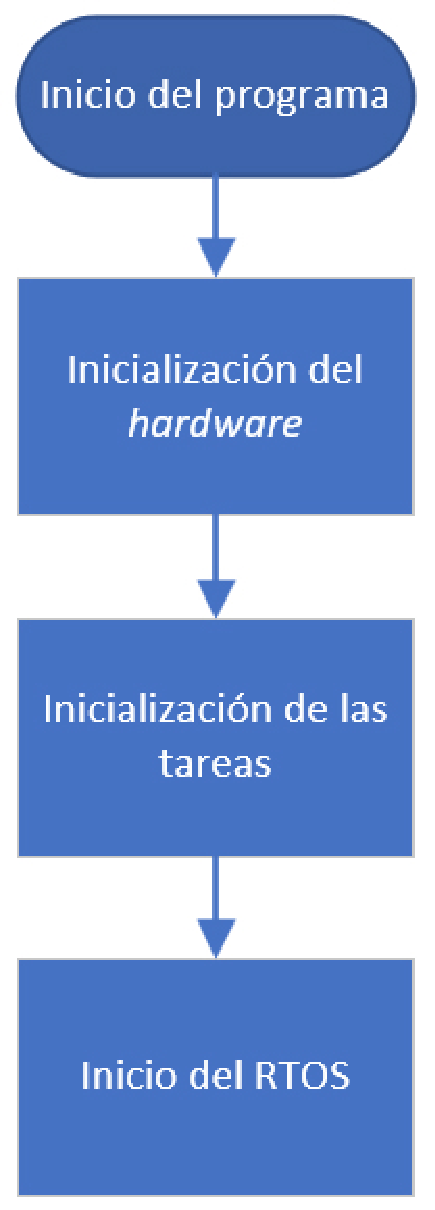
\includegraphics[height=0.5\textheight]{arch_bucle}
  \caption{Bucle principal del \sw{}} \label{fig:bucle}
\end{figure}

\begin{figure}[!h]
  \centering
  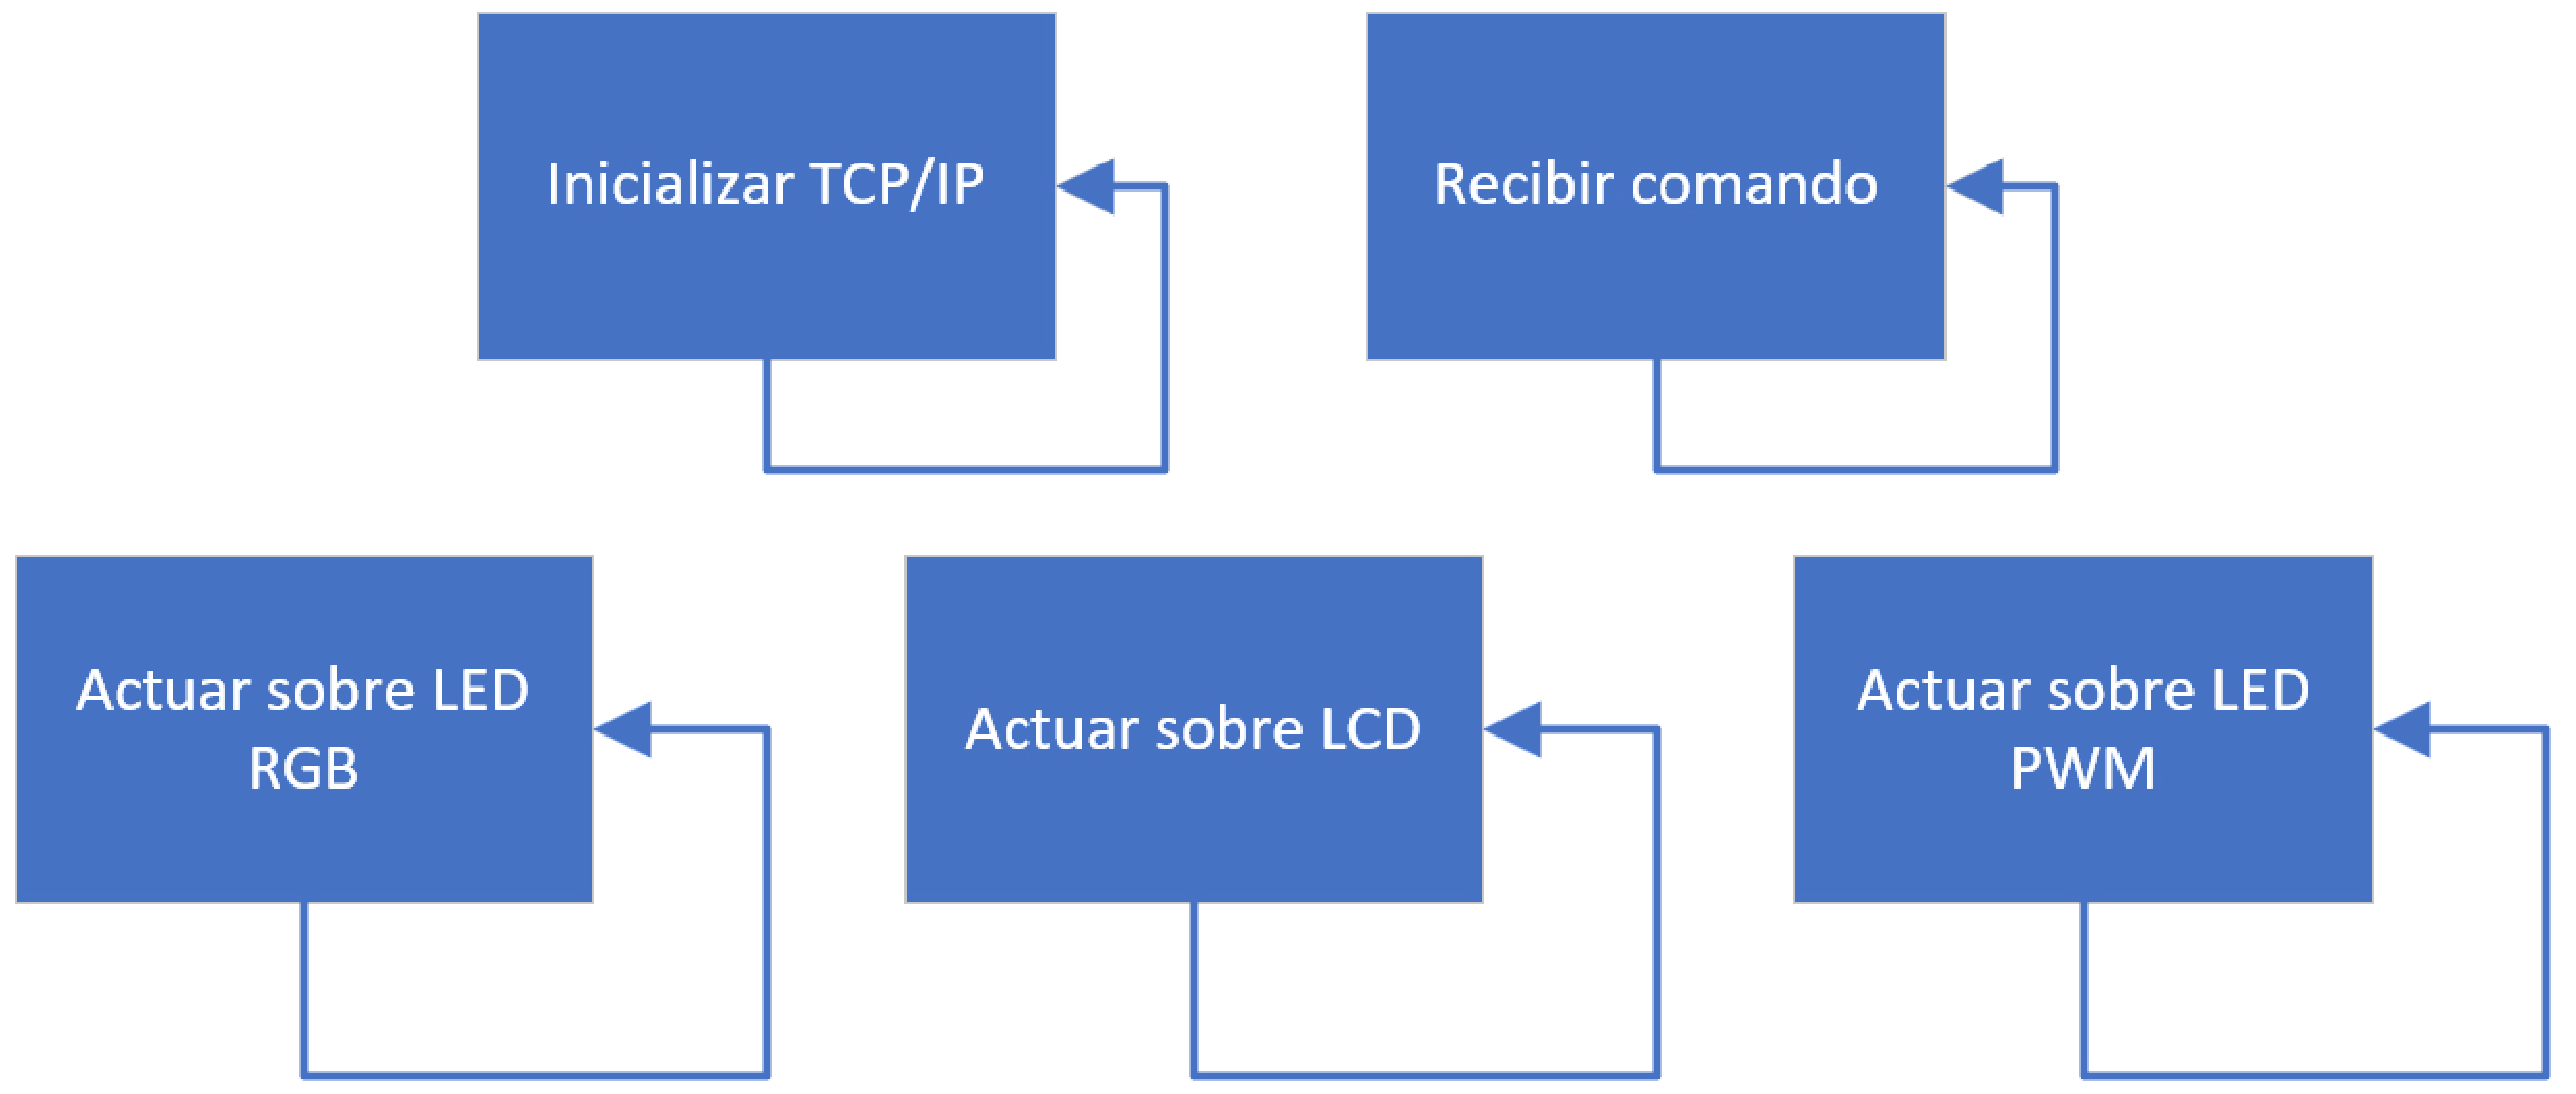
\includegraphics[width=0.6\textheight]{arch_tareas}
  \caption{Tareas para el RTOS} \label{fig:tareas}
\end{figure}

Con las tareas \ref{fig:tareas} se da respuesta a los casos de usos planteados
para el sistema empotrado durante la especificación de los requisitos del \sw{}.
Gracias la flexibilidad que aporta esta solución se podrían añadir o remover
funciones rápidamente. Por ejemplo, bastaría con agregarlas o quitarlas del 
RTOS durante la inicialización \ref{fig:bucle}.


\subsection{Diseño arquitectónico de la aplicación web} \label{sec:arch-aw}
Por lo que se refiere al \sw{} de aplicación web, representa un cambio de
contexto completo. La aplicación se encuentra alojada en un servidor de
aplicaciones que permite al usuario acceder a la interfaz web desde un
navegador web cualquiera.

La tecnología a utilizar en conjunción con el servidor de aplicaciones es
JavaServer Faces (JSF) \cite{webpage:jsf}. Su especificación concreta su
propósito para construir aplicaciones web e interfaces de usuarios basadas
en componentes. Cada componente de \sw{} sirve para encapsular un conjunto
de funciones o datos estrechamente relacionados.

Además, JSF utiliza el patrón de arquitectura Modelo-Vista-Controlador (MVC).
Este patrón separa la lógica de la aplicación en tres componentes diferenciados.
Con la separación se impulsa el desarrollo modular, facilitando la colaboración
y la reutilización durante el desarrollo.

Los tres componentes de MVC son:
\begin{description}
  \item[Modelo:] Define los datos y su estructura empleados por la aplicación.
  Si los datos se modifican, la vista se actualiza para reflejar los cambios.
  \item[Vista:] Define la interfaz y como se muestran los datos al usuario
  en ella.
  \item[Controlador:] Contiene la lógica responsable de manipular el modelo
  en función de las acciones del usuario.
\end{description}

\imagenancho{arch_mvc}{Relación entre MVC y el usuario}{!h}{0.8}

\subsubsection{Diseño del modelo} \label{sec:arch-modelo}
En JSF el modelo se define mediante \extranjerismo{beans}. Los
\extranjerismo{beans} se crean con clases Java. Están compuestos por una
conjunto de atributos y sus correspondientes métodos 
\extranjerismo{getters} y \extranjerismo{setters}.

Así pues, el valor de un atributo, también llamado propiedad, se consulta con
su correspondiente método \extranjerismo{get} y se puede actualizar con su
método \extranjerismo{set}.

\subsubsection{Diseño de la vista} \label{sec:arch-vista}
En JSF la vista se define mediante ficheros escritos en Extensible HyperText
Markup Language (XHTML) que incluyen etiquetas especiales para añadir
componentes específicos de JSF. Posteriormente, el código de los ficheros XHTML
es traducido a código Hypertext Markup Language (HTML) interpretable por los
navegadores web.

La conexión entre la interfaz y el resto de la aplicación se realiza con ayuda
del Lenguaje de Expresiones de JSF (EL). Con estas expresiones se enlazan los
componentes de la interfaz con las propiedades de los \extranjerismo{beans}.

\subsubsection{Diseño del controlador} \label{sec:arch-ctl}
En JSF el controlador se puede definir con \extranjerismo{beans} al igual
que en el modelo \ref{sec:arch-modelo}. Pero a diferencia de los
\extranjerismo{beans} del modelo, los \extranjerismo{beans} del controlador
cuentan con los métodos necesarios para realizar la lógica de negocio
requerida por la aplicación.


\subsection{Diseño conjunto del sistema} \label{sec:design-comp}

\imagenancho{componentes}{Diagrama de componentes del sistema}{!h}{1}


\subsection{Diagramas de clases} \label{sec:design-comp}

\imagenancho{pkg-controller}{Diagrama de clases de los paquetes
\extranjerismo{controller} y \extranjerismo{controller.network}}{H}{0.9}

\imagenalto{pkg-model}{Diagrama de clases del paquete
\extranjerismo{model}}{H}{0.3}


\subsection{Diseño de la interfaz} \label{sec:design-iface}
Para que el usuario pueda controlar el sistema empotrado, la aplicación web
pone su disposición una interfaz web. En una sola página el usuario puede
ver las funciones disponibles y operar con ellas.

En primer lugar la interfaz tiene que permitir que el usuario introduzca
los datos de conexión con el sistema empotrado.

\imagenancho{panel_datos}{Introducción de datos}{!h}{0.9}

Una vez establecidos los datos se muestran unos paneles con las funciones
disponibles.

Con unos botones se puede escoger el color iluminado por los LED RGB.

\imagenancho{panel_led}{Panel para cambiar el color de los LED RGB}{!h}{0.9}

En unos cuadros de texto, el usuario puede introducir un mensaje y pulsando
un botón lo puede enviar.
\imagenancho{panel_msg}{Panel para enviar un texto al LCD}{!h}{0.9}

\clearpage

Con unos controles deslizantes, el usuario puede cambiar la intensidad del brillo
de los LED regulados por PWM.
\imagenancho{panel_pwm}{Panel para regular el brillo de los LED PWM}{!h}{0.9}

\clearpage

La interfaz completa se construye según lo definido en el siguiente diseño.

\begin{figure}[H]
  \centering
  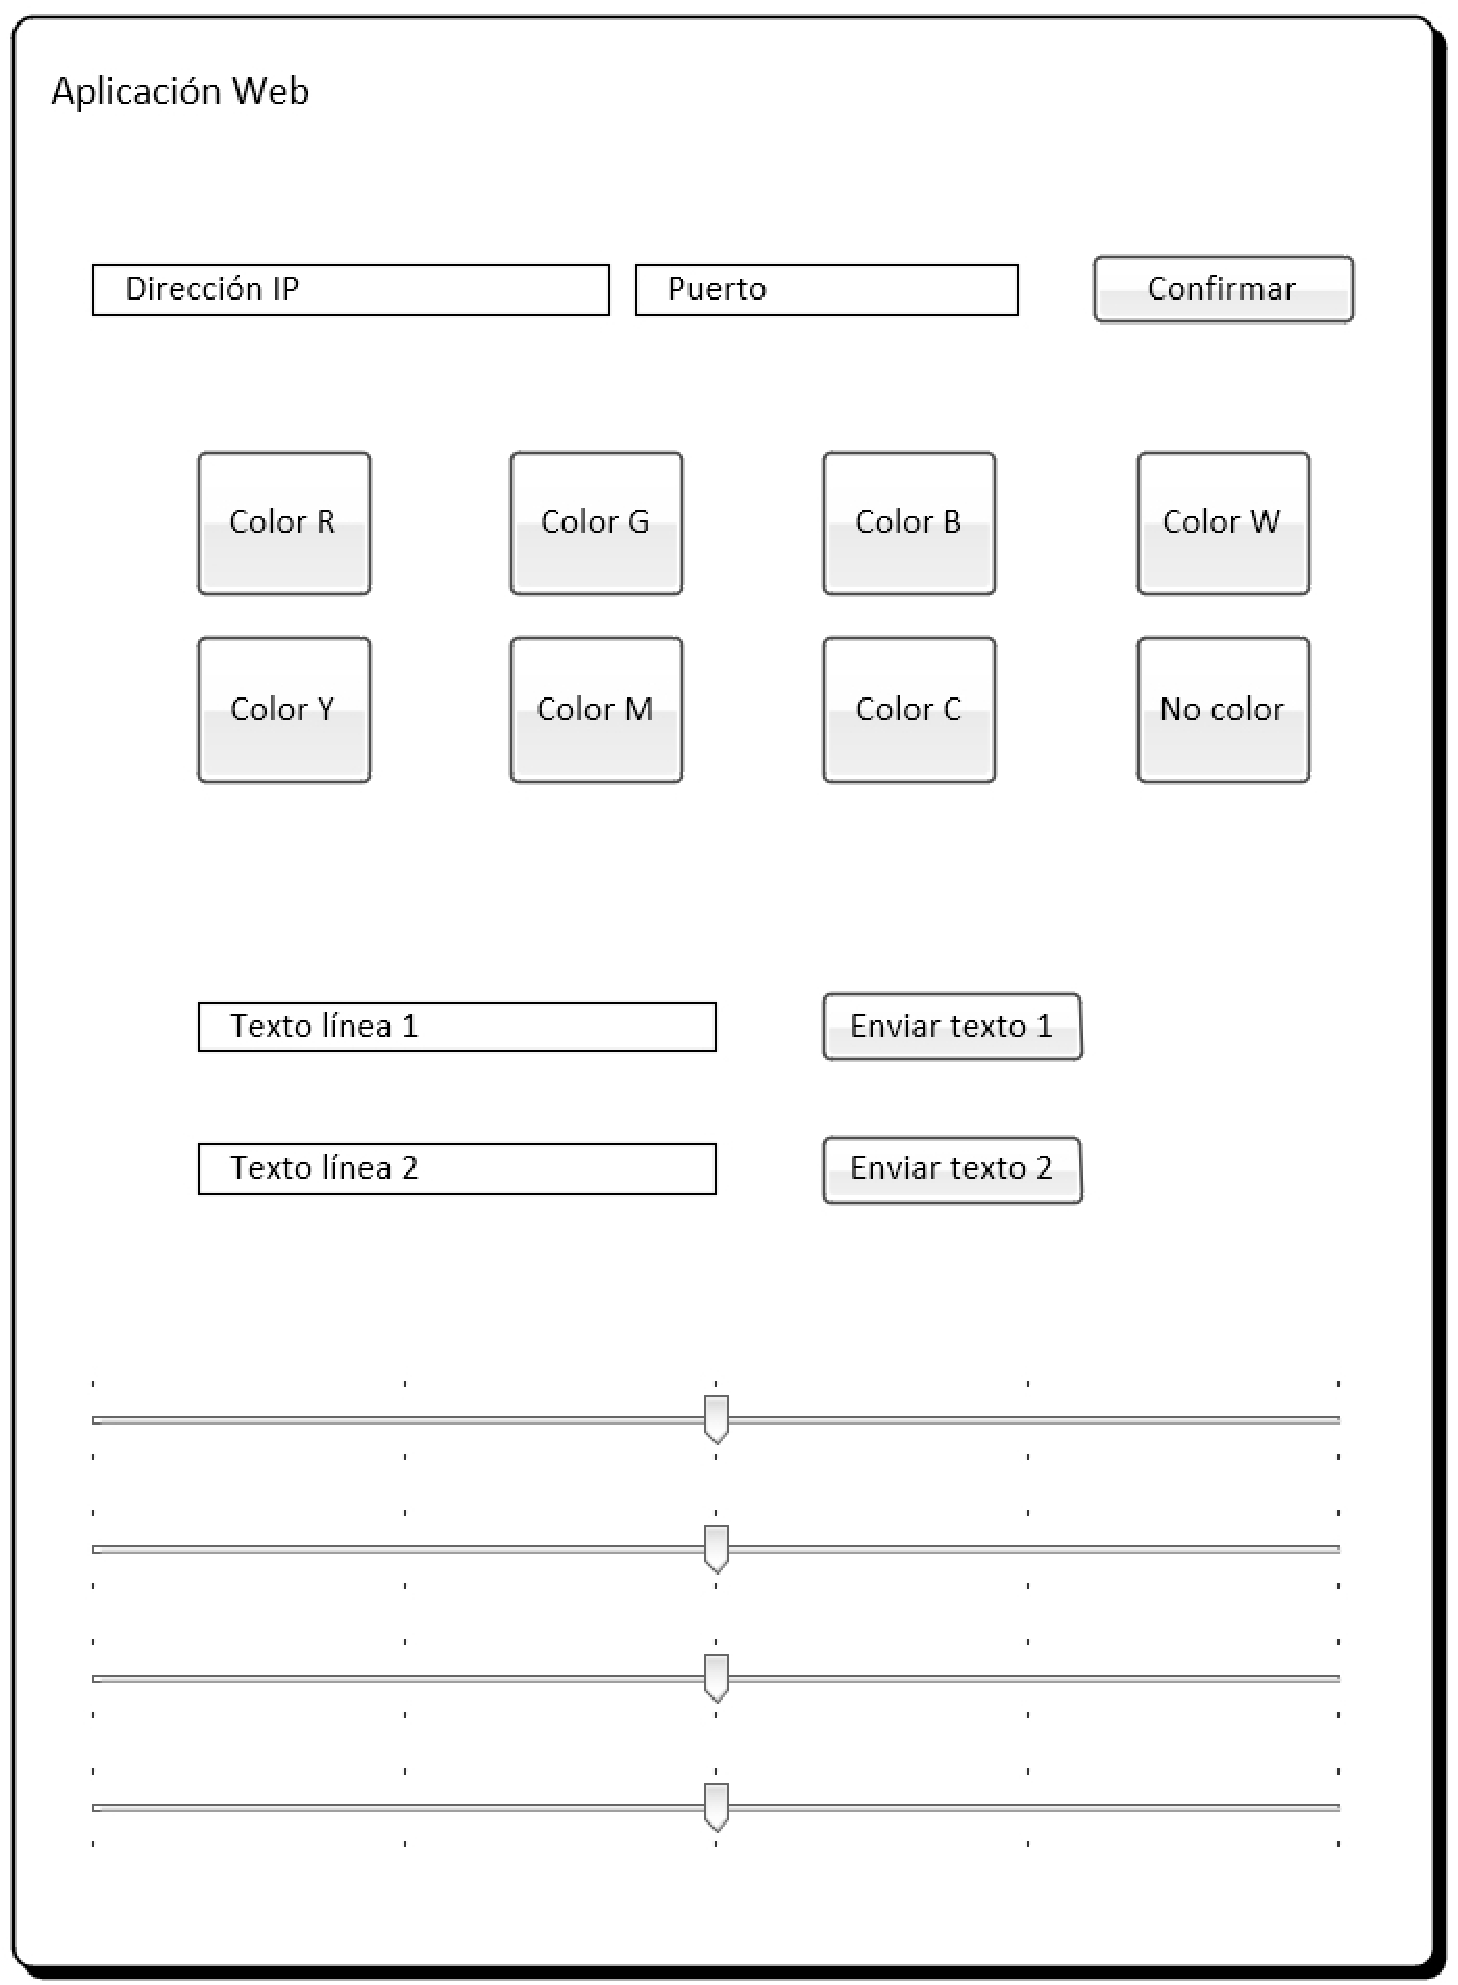
\includegraphics[width=0.55\textheight]{interfaz}
  \caption{Diseño de la interfaz} \label{fig:intefaz}
\end{figure}

\clearpage

\section{Diseño procedimental} \label{sec:design-proc}
El siguiente diagrama muestra las interacciones que se producen entre
los componentes del sistema desde que el usuario solicita una función hasta que
el sistema empotrado la realiza.

\figuraApaisadaSinMarco{0.9}{secuencia}{Diagrama de secuencia}{fig:secuencia}{}

\apendice{Documentación técnica de programación} \label{ch:man-dev}

\section{Introducción} \label{sec:man-dev-intro}
Para que cualquier persona interesada en conocer, modificar o extender
el sistema desarrollado, este apéndice muestra los aspectos a tener en cuenta
para lograrlo.

Como los componentes del sistema, el sistema empotrado y la aplicación web,
tienen características tan diferentes cada uno necesita herramientas específicas
para su desarrollo.

Se detallan las particularidades de cada herramienta, los ajustes de
configuración, la estructura que toman los directorios con los ficheros
y los pasos necesarios para poner en funcionamiento el proyecto.



\section{Estructura de directorios} \label{sec:man-dev-struct}
Para empezar a trabajar con el proyecto lo primero que se necesita es una
copia del código fuente. La manera más sencilla de consultar y obtener el código
es acudir a los repositorios de GitHub. Hay un repositorio dedicado al \sw{}
del sistema empotrado \cite{webpage:repo-se} y otro para el \sw{} de la
aplicación web \cite{webpage:repo-aw}.


\subsection{Estructura de directorios del sistema empotrado}
\label{sec:man-dev-struct-se}
El código fuente del \sw{} del sistema empotrado toma la siguiente estructura:

\begin{description}
  \item[/] Directorio raíz, contiene el resto de directorios. Incluye el
  fichero LICENSE que contiene los términos y condiciones del licenciamiento
  del \sw{}. Además contiene un fichero de tipo ``mex'' generado por el entorno
  de desarrollo (IDE) que sirve para configurar el \hw{} de la placa de
  desarrollo. Y el fichero Doxyfile que configura la herramienta de documentación.
  \item[/CMSIS/] Fuentes pertenecientes al Cortex Microcontroller Software
  Interface Standard (CMSIS). Proporciona interfaces al procesador y sus
  periféricos.
  \item[/amazon-freertos/] Fuentes pertenecientes a FreeRTOS, el RTOS usado por
  el sistema empotrado.
  \item[/board/] Fuentes autogenerados por el IDE y sus Config Tools que 
  permiten habilitar y configurar el \hw{} de la placa de desarrollo.
  \item[/doc/] Contiene la documentación del código y del proyecto.
  \item[/doc/amazon-freertos/] Documentación incluida con FreeRTOS.
  \item[/doc/lwip/] Documentación incluida con lwIP.
  \item[/doc/memoria/] Documentación del proyecto, la memoria descriptiva junto
  con sus apéndices.
  \item[/doc/html] Documentación del código fuente generada por Doxygen.
  \item[/drivers/] Fuentes con los controladores necesarios para trabajar con el
  \hw{}.
  \item[/lwip/] Fuentes relativos a lwIP, la implementación de la pila de 
  protocolos TCP/IP.
  \item[/source/] Código fuente del proyecto. A destacar, el fichero ``main.c''
  encargado del funcionamiento general del sistema. Están presentes los ficheros
  encargados de tratar con \hw{}. También se encuentran los ficheros de
  configuración.
  \item[/startup/] Código de arranque generado por el IDE.
  \item[/utilities/] Código generado por el IDE con utilidades auxiliares usadas
  para depuración o registro de eventos.
\end{description}


\subsection{Estructura de directorios de la aplicación web}
\label{sec:man-dev-struct-aw}
El código fuente del \sw{} de la aplicación web toma la siguiente estructura:

\begin{description}
  \item[/] Directorio raíz, contiene el resto de directorios. Aquí se ubica el
  fichero ``pom.xml'' usando por la herramienta Maven para la gestión y
  construcción del proyecto.
  \item[/doc/] Documentación del código fuente generada por Javadoc.
  \item[/src/main/] Contiene todo el código perteneciente a la aplicación web.
  \item[/src/main/java/] Código Java que implementa la lógica de negocio.
  \item[/src/main/webapp/] Contiene el fichero XHTML con el código de la
  interfaz web.
  \item[/src/main/webapp/WEB-INF] Contiene los ficheros XML usados por
  el servidor de aplicaciones.
  \item[/src/main/webapp/resources/] Recursos adicionales de la interfaz web.
  \item[/src/main/webapp/resources/css/] Contiene el fichero CSS que modifica el
  aspecto de la interfaz.
  \item[/src/main/webapp/resources/images/] Contiene las imágenes y otros
  recursos gráficos a usar en la interfaz.
\end{description}



\section{Manual del programador}
Para desarrollar el proyecto se han utilizado dos IDE diferentes, uno para cada
\sw{}. Aunque no es indispensable usar las mismas herramientas, a continuación
se muestra como obtener, instalar, configurar y utilizarlas de la misma
manera que se ha hecho durante el proyecto.


\subsection{MCUXpresso IDE} \label{sec:man-dev-mcuxpresso}

\subsubsection{Instalación de MCUXpresso IDE} \label{sec:instalacion-mcu}
El IDE se puede obtener gratuitamente desde la zona de Recursos para
desarrolladores de NXP \cite{webpage:mcuxpresso-ide}. El único requisito
establecido por NXP es tener una cuenta registrada, gratuita también, en su
sitio web.

Una vez iniciada la sesión y accedido al área de descarga se puede obtener
la versión más reciente del IDE. De ser necesario, también es posible descargar
una versión antigua desde la pestaña \extranjerismo{Previous}.

Tras aceptar los términos y condiciones de uso se muestran los enlaces de
descarga de los instaladores del IDE. 

\imagen{mcu_descarga}{Descarga de MCUXpresso IDE}

El instalador sigue el proceso de instalación habitual a la mayoría de programas.
Aceptar licencia de uso, indicar la ubicación del programa e informar
que se van a instalar controladores de depuración son los pasos más relevantes.

Concluida la instalación MCUXpresso solicita la ubicación del espacio de trabajo
o \extranjerismo{workspace} donde situar los proyectos. Cuando MCUXpresso
está listo para su uso presenta el aspecto habitual a cualquier otro IDE basado
en Eclipse IDE.

\imagen{mcuxpresso-wsp}{MCUXpresso recién instalado}

\subsubsection{Instalación de MCUXpresso SDK} \label{sec:instalacion-mcu}
MCUXpresso IDE lleva integrado las MCUXpresso Config Tools, sin embargo, es
necesario instalar MCUXpresso SDK, el kit de desarrollo de software (SDK),
que incluye los \extranjerismo{drivers}, \extranjerismo{middleware} y otras
utilidades necesarias para el desarrollo.

Las características del SDK están descritas en la web de NXP
\cite{webpage:mcuxpresso-sdk} al igual que las de MCUXpresso IDE. En cambio,
la descarga se realiza desde un sitio dedicado a la configuración de los SDK.

\imagen{sdk-download}{Sitio de MCUXpresso SDK Builder
\cite{webpage:mcuxpresso-sdk-builder}}

El sitio de configuración de SDK permite personalizar, o construir, un SDK
específico para la placa de desarrollo utilizada. Además permite seleccionar
que componentes incluir o no en el SDK.

Para poder descargar el SDK, NXP requiere iniciar sesión con una cuenta de
usuario de la misma manera que en la descarga del MCUXpresso IDE.

Dentro del configurador, el primer paso necesario consiste en buscar el
\hw{} para el que está destinado el SDK. En este caso, el \hw{} de desarrollo
va a ser la placa de desarrollo FRDM-K64F.

\imagen{sdk-selector}{Selección de la placa de desarrollo
\cite{webpage:mcuxpresso-sdk-builder}}

Seleccionada la placa de desarrollo falta configurar el SDK a las necesidades
del proyecto. La elección del sistema operativo puede variar entre
desarrolladores por lo que queda en su mano la elección. Por otro lado, el IDE
va a ser necesariamente MCUXpresso IDE.

Por último, hay que configurar el \extranjerismo{middleware} incluido con el SDK.
Los componentes mínimos a seleccionar son FreeRTOS y lwIP aunque no supone
ningún inconveniente elegir más componentes.

\imagen{full-sdk}{Resumen del SDK completo
\cite{webpage:mcuxpresso-sdk-builder}}

MCUXpresso IDE ofrece una vista con los SDK instalados. Para agregar el SDK
recién descargado basta con hacer clic derecho en dicha vista e importar el
fichero comprimido con el SDK. Como alternativa, también sirve arrastrar el
fichero a la vista para para importar el SDK.

\imagen{sdk-import}{Importación del SDK}

\imagen{sdk-imported}{Detalles del SDK correctamente importado}

\subsubsection{Importación del proyecto} \label{sec:importacion-proj}
Para empezar a trabajar con el proyecto falta importar una copia el código
fuente. Una opción consiste en importar el proyecto directamente desde una
carpeta con los ficheros o desde un fichero con el proyecto comprimido.

Copiarlo desde un repositorio es otra opción que permite obtener la versión
del código más reciente. El código del \sw{} del sistema empotrado se halla en
GitHub \cite{webpage:repo-se}.

\begin{figure}[!h]
  \centering
  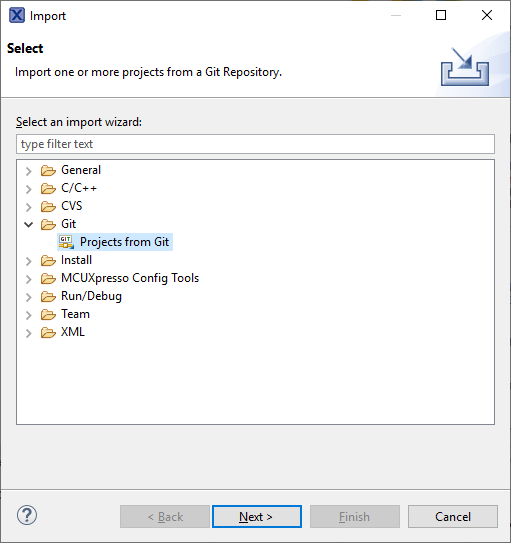
\includegraphics[height=0.45\textheight]{import}
  \caption{Importación del proyecto desde GitHub} \label{fig:import}
\end{figure}

La introducción de credenciales es necesaria para poder realizar
\extranjerismo{commit}, \extranjerismo{push} y el resto de operaciones de Git
con destino a GitHub, siempre y cuando se tengan permisos para operar en el
repositorio. Sino, solo se puede trabajar en local.

\begin{figure}[!h]
  \centering
  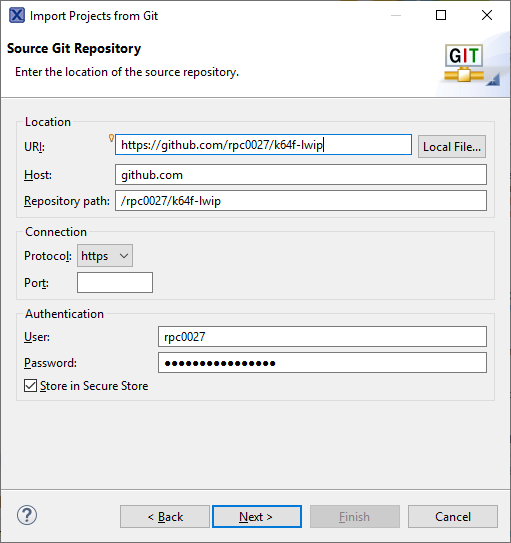
\includegraphics[height=0.45\textheight]{clone-git}
  \caption{Datos del repositorio} \label{fig:clone-git}
\end{figure}

Al aceptar la conexión con el repositorio, una serie de ventanas solicita más
información respecto a la ubicación del repositorio local, el proyecto a 
importar y si el proyecto se importa directamente o no.

Completado el proceso de importación el proyecto se encuentra listo 
trabajar con él.

\begin{figure}[!h]
  \centering
  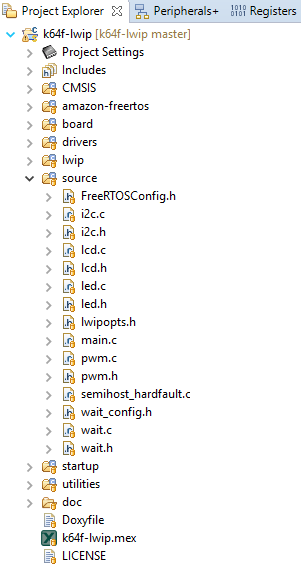
\includegraphics[height=0.45\textheight]{project-ready}
  \caption{Proyecto correctamente importado} \label{fig:project-ready}
\end{figure}

\subsubsection{Vista general de las Config Tools} \label{sec:config-tools}
Uno de los elementos diferenciadores de MCUXpresso respecto a IDE anteriores
es la incorporación de las Config Tools o herramientas de configuración.

En concreto, son tres herramientas que permiten configurar tres componentes
del sistema: pines, relojes y periféricos. Además, generan automáticamente el
código oportuno para habilitar e inicializar los dispositivos configurados. El
acceso a estas herramientas se consigue cambiando a sus respectivas perspectivas.

Con Pin Tools se configuran los pines del microcontrolador (MCU) enrutando
sus pines con la salida o la entrada adecuada. Los pines se pueden seleccionar y
enrutar en la vista ``Pins'' de la herramienta. Además, Pin Tools permite asociar
los pines en grupos. De esta manera es posible habilitar e inicializar grupos
de pines concretos simultáneamente.

\imagen{pin_selector}{Pines del grupo Ethernet en verde brillante}

Algunos pines requieren configuración adicional que se puede ajustar en la vista
``Routed Pins''.

\imagen{pin_config}{Configuración de los pines del grupo Ethernet}

La herramienta Clock Tools se utiliza para configurar los relojes del sistema
empotrado. En la vista ``Clocks Table'' se pueden introducir los valores de
configuración: frecuencias, multiplicadores, divisores... Por otra parte, la
vista ``Clocks Diagram'' muestra de forma gráfica la configuración establecida
en ese momento, aunque también permite cambiar los ajustes sobre el diagrama
directamente.

\figuraApaisadaSinMarco{0.9}{clocks_diag}{Diagrama con los relojes del sistema}
{fig:relojes}{}

La última herramienta, Peripheral Tools, posibilita la configuración de los
dispositivos periféricos conectados al MCU. En función del periféricos se
muestras las opciones específicas para cada uno de ellos.

\imagen{peripherals}{Configuración del periférico FTM}


\subsection{Eclipse IDE} \label{sec:man-dev-eclipse}
El desarrollo de la aplicación web requiere de varias herramientas aparte
del propio IDE. Una es el kit de desarrollo de Java, JDK, y la otra es el
SDK de Java EE. Además, como se usa Maven para la gestión del proyecto, también
es necesaria su instalación.

\subsubsection{Instalación de JDK} \label{sec:jdk}
El JDK se puede obtener de la zona de descargas de Oracle \cite{webpage:javaee}.
Como el JDK es utilizado por el resto de herramientas, su descarga e instalación
se debe realizar en primer lugar. El instalador se encarga de todo el proceso a
excepción de la creación de dos variables de entorno.

Para poder usar el JDK desde la consola de comandos, es necesario crear
una variable de entorno llamada ``JAVA\_HOME'' que apunte al directorio de
instalación del JDK. Después, hay que modificar el ``PATH'' al que hay
que añadir la nueva variable.

\subsubsection{Instalación de Maven} \label{sec:maven}
Maven está disponible en su sitio web \cite{webpage:maven}. La descarga consiste
en un fichero comprimido que no contiene ningún instalador. Para su uso, basta
con descomprimir el fichero en algún directorio del sistema. Después, para
localizar el directorio hay que crear una variable de entorno al igual que con
el JDK. En este caso, la varible se tiene que llamar ``M2\_HOME'' y también
hay que agregarla al ``PATH''.

\subsubsection{Instalación de GlassFish} \label{sec:glassfish}
La manera de instalar GlassFish es similar a la anterior. Hay que descargar un
fichero comprimido desde su sitio web \cite{webpage:glassfish}, descomprimir
el fichero en un directorio a elegir y que crear una variable que apunte a ese
directorio. En este caso, la variable de entorno toma el nombre de 
``GLASSFISH\_HOME'' y también se añade al ``PATH''.

\subsubsection{Instalación de Eclipse IDE} \label{sec:eclipse}
El instalador del IDE se puede obtener libremente desde el sitio de Eclipse
\cite{webpage:eclipse}. Como existen varias versiones de Eclipse, el instalador
permite escoger la versión requerida, en este caso, se selecciona ``Eclipse IDE
for Enterprise Java Developers''.

\imagen{installer}{Instalador de Eclipse IDE}

Después de terminar la instalación de Eclipse, es necesario instalar
una pequeña herramienta llamada Eclipse GlassFish Tools capaz de conectar el
GlassFish con Eclipse. De esta manera es posible publicar las aplicaciones web y
controlar el estado del servidor directamente desde el IDE.

La herramienta se encuentra disponible tanto en el Eclipe Marketplace como
en el repositorio de la propia herramienta \cite{webpage:glassfish-tools}. Una
vez instalada, se puede configurar el servidor desde la vista ``Servers''.

\imagen{repository}{Instalación de las Eclipse GlassFish Tools}

\subsubsection{Importación del proyecto} \label{sec:importacion-proj-ee}
La importación del proyecto es similar a la descrita para MCUXpresso
\ref{sec:importacion-proj}, bien importando un fichero o bien descargándolo
desde GitHub \cite{webpage:repo-aw}.

\begin{figure}[!h]
  \centering
  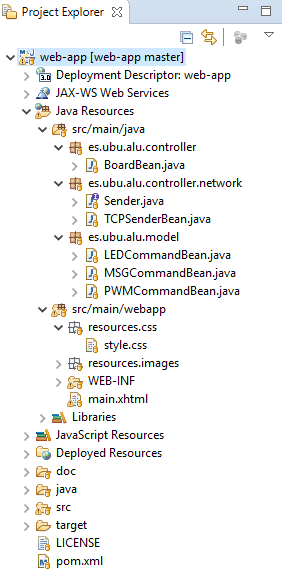
\includegraphics[height=0.45\textheight]{aw-imported}
  \caption{Proyecto correctamente importado} \label{fig:aw-imported}
\end{figure}

\clearpage



\section{Compilación, instalación y ejecución del proyecto} \label{sec:exe}
Con los entornos de desarrollo y sus respectivos proyectos preparados es posible
compilar los códigos fuente. Dependiendo del \extranjerismo{software} a ejecutar
es necesario tomar diferentes caminos para su puesta en marcha.


\subsubsection{Compilación, escritura y ejecución del sistema empotrado}
\label{sec:exe-se}
Existen varias vías para compilar el código fuente. Una de ellas es hacer clic
derecho sobre el proyecto y en el menú contextual, pulsar sobre ``Build
Project''. Otra forma es pulsar sobre su icono en la barra de herramientas.

Para realizar la escritura, o \extranjerismo{flash}, de los binarios en el
sistema empotrado y que pueda ejecutarlos hay que lanzar desde el IDE la
operación de ``Debug''. Igual que la compilación, se puede hacer desde el menú
contextual o desde la barra de herramientas. Cabe decir que la operación de
depuración ejecuta automáticamente la de compilación, haciendo innecesario tener
que ordenarla manualmente.

La primera vez que se lanza un \extranjerismo{debug} el IDE solicita la
identificación de la placa de desarrollo. Para identificar la placa de
desarrollo hay que especificar el uso de ``SEGGER J-Link probes'', 
compatibles con OpenSDA, el adaptador serie y de depuración integrado en la
placa. 

\imagen{probes}{Reconocimiento de la placa de desarrollo}

\imagen{probed}{Placa de desarrollo reconocida}

Cuando la placa dispone del \sw{} arranca su ejecución. Al estar en modo de
depuración, la consola de depuración se activa y queda lista para mostrar los
mensajes enviados por la placa cuando corresponda.

\imagen{console}{Sistema en ejecución}


\subsubsection{Despliegue y ejecución de la aplicación web} \label{sec:exe-aw}
Como la aplicación web depende de un servidor de aplicaciones para funcionar,
se hace necesario desplegarla en uno antes de poder utilizarla.

Eclipse junto con la herramienta GlassFish Tool \ref{sec:eclipse} permite
realizar el despliegue automáticamente. Además, permite controlar el servidor
de aplicaciones pudiendo iniciarlo, detenerlo o incluso, actualizar los
ficheros de una aplicación ya desplegada.

En la vista ``Servers'' y haciendo clic derecho sobre el servidor GlassFish
se puede desplegar la aplicación pulsando en la opción ``Add and remove'' del
menú contextual. En la ventana que aparece después, se selecciona la aplicación
en el cuadro de la derecha y pulsando ``Add >'' queda configurada para ser
publicada en el servidor.

\begin{figure}[!h]
  \centering
  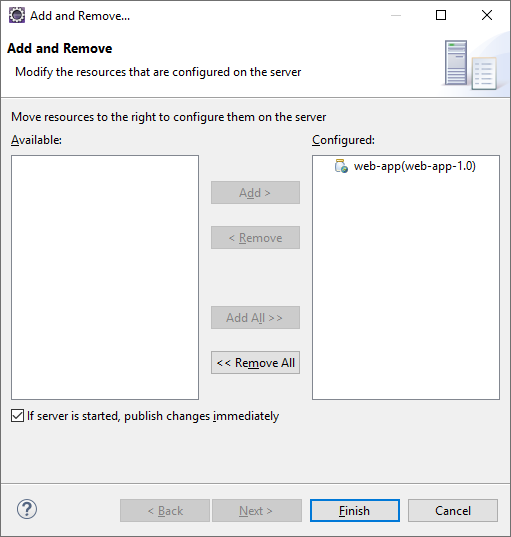
\includegraphics[height=0.45\textheight]{add}
  \caption{Aplicación configurada para ser publicada} \label{fig:add}
\end{figure}

Mientras el código de la aplicación no sea modificado, la aplicación tendrá el
estado de sincronizada. Si el código cambia, su estado indicará que necesita
ser vuelta a publicar.

\begin{figure}[!h]
  \centering
  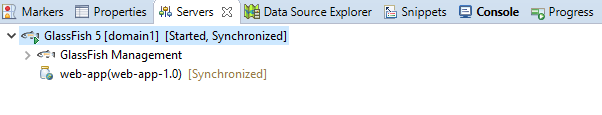
\includegraphics[width=0.6\textwidth]{published}
  \caption{Aplicación publicada} \label{fig:publicada}
\end{figure}

Si el despliegue se ha completado con éxito, ya es posible acceder a la
aplicación web desde un navegador cualquiera. La URL de la aplicación es:
http://localhost:8080/web-app/ .

\imagen{success}{Acceso a la aplicación web desde un navegador}

Con Maven se presenta otra forma de abordar la construcción y publicación de la
aplicación web. Ejecutando en el directorio raíz del proyecto el comando:
\begin{quotation}
  mvn package
\end{quotation}
Maven crea un archivo de tipo WAR, utilizados en Java para la distribución de
aplicaciones web, llamado ``web-app-1.0.war''. Ese archivo se puede publicar
en el servidor con el siguiente comando:
\begin{quotation}
  asadmin deploy web-app-1.0.war
\end{quotation}
En caso de que la aplicación ya estuviera desplegada, por ejemplo, porque se ha
desplegado desde Eclipse, el comando fallaría avisando de esta circunstancia.
De no haber errores, la aplicación web queda disponible para ser utilizada
usando la misma URL que en el caso anterior. 



%\section{Pruebas del sistema}
\apendice{Documentación de usuario} \label{ch:man-user}



\section{Introducción} \label{sec:man-user-intro}
Para que cualquier persona interesada pueda usar el sistema desarrollado,
este apéndice muestra los pasos necesarios.

Se indican los requisitos para la puesta en marcha del sistema empotrado
y de la aplicación web. También se indican las instrucciones para su correcta
instalación. Por último, un pequeño manual explica brevemente las funciones
accesibles desde la aplicación web.



\section{Requisitos de usuarios} \label{sec:man-user-req}
Como el sistema está compuesto por el sistema empotrado y por la aplicación web
es requisito fundamental tener ambos componentes listos para su utilización
por parte del usuario.


\subsection{Requisitos del sistema empotrado} \label{sec:man-user-req-se}
El sistema empotrado debe contar con el \sw{} almacenado en su memoria. En caso
de no estarlo, se deben seguir los pasos descritos en el apéndice con la
Documentación técnica de programación \ref{ch:man-dev}, en concreto, la sección
dedicada a la Compilación, escritura y ejecución del sistema empotrado
\ref{sec:exe-se}.


Para que el sistema empotrado pueda solicitar y recibir una dirección IP se
utiliza el protocolo DHCP. Por lo tanto, se requiere de la presencia de un
servidor DHCP en la red. Habitualmente, los \extranjerismo{routers} usados
en redes pequeñas de tipo residenciales o Small Offices/Home Offices (SOHO)
llevan incluido un servidor DHCP facilitando la instalación al usuario.


\subsection{Requisitos de la aplicación web} \label{sec:man-user-req-aw}
La aplicación web es accesible desde cualquier navegador web. Se puede usar
cualquiera de los dispositivos habituales usados para acceder a la web. Bien
sean equipos de sobremesa o sean dispositivos móviles.

Como la aplicación se ejecuta en un servidor de aplicaciones, es necesario
contar con uno en la misma red donde se conecta el sistema empotrado. Las
instrucciones sobre como desplegar la aplicación se detallan en el apéndice
con la Documentación técnica de programación \ref{ch:man-dev}, en concreto, la
sección dedicada a la Compilación, escritura y ejecución de la aplicación web
\ref{sec:exe-aw}.



\section{Instalación} \label{sec:man-user-inst}
Si se cumplen los requisitos anteriores, la instalación se reduce a conectar y
arrancar el sistema empotrado.

Para establecer la conexión a la red basta con un cable de par trenzado
conectado al sistema empotrado en un extremo y a un \extranjerismo{switch},
\extranjerismo{router} u otro dispositivo de acceso a la red en el
otro.

Para finalizar, el arranque del sistema empotrado se realiza automáticamente
cuando se conecta un cable USB en alguno de sus puertos Micro-USB. Esta conexión
se encarga de suministrar la alimentación eléctrica al sistema.

\imagenancho{boot}{Arranque del sistema empotrado}{!h}{0.6}

Una vez encendido, el sistema empotrado solicitará una dirección IP. Tras
obtenerla, la mostrará por pantalla junto al puerto TCP abierto.
Cuando se muestran estos datos ya es posible enviar instrucciones al sistema
empotrado desde la aplicación web.



\section{Manual del usuario} \label{sec:man-user}
La aplicación web está accesible desde la URL http://servidor:8080/web-app/,
siendo ``servidor'' la dirección del servidor de aplicaciones.

\imagenancho{landing}{Vista general de la web}{!h}{0.9}

Los botones de la barra de navegación permiten desplazarse directamente a las
funciones.

\imagenancho{navigation}{Barra de navegación}{!h}{0.75}

Para poder transmitir las instrucciones al sistema empotrado hay que indicar
los ajustes de red. Por defecto se muestra un ejemplo del tipo de direcciones
habitual en redes locales y el puerto TCP usado durante el desarrollo.

\imagenancho{network}{Ajustes de red iniciales}{!h}{0.75}

Estos datos los proporciona el sistema empotrado tras su arranque. 

\imagenancho{dhcp}{IP y puerto del sistema empotrado}{!h}{0.6}

Tras escribir los datos, pulsando conectar la aplicación web queda preparada
para comunicarse con ese sistema empotrado.

\imagenancho{network2}{Ajustes de red establecidos}{!h}{0.75}

La primera función disponible es el encendido de las luces de colores usando
los LED RGB. El color de cada botón refleja el color de la luz a mostrar.
En cambio, pulsando el negro se apagan todos los LED encendidos.

\imagenancho{rgb}{Colores iluminables con los LED RGB}{!h}{0.75}

La segunda función muestra cadenas de caracteres en la pantalla LCD del sistema
empotrado. Para cada línea del LCD se proporciona un cuadro de texto diferente.
Cada cuadro se acompaña de un botón para confirmar el envío del mensaje.

\imagenancho{msg}{Envío de mensajes a la pantalla LCD}{!h}{0.75}

Por ejemplo, enviando el texto que aparece por defecto la pantalla de sistema
empotrado la muestra de la siguiente manera. \footnote{Como el texto por defecto
supera el límite de 16 caracteres del LCD, la última palabra se descarta.}

\imagenancho{msg-lcd}{Mensajes enviados a la pantalla LCD}{!h}{0.6}

La tercera y última función disponible es la regulación de la intensidad del
brillo de unos LED mediante PWM. Para realizar esta regulación se muestran 
cuatro controles deslizantes de colores. Cada uno con el color del LED que
regula.

\imagenancho{pwm}{Controles deslizantes para los LED PWM}{!h}{0.8}

Todos los controles parten de la posición inicial de apagado (o 0\%).
Deslizándolos a derecha e izquierda se puede ajustar al valor que se quiera.

\imagenancho{pwm2}{Controles ajustados a diferentes valores}{H}{0.8}



\bibliographystyle{plain}
\bibliography{bibliografiaAnexos}

\end{document}
